\documentclass{article}
\usepackage[utf8]{inputenc}
\usepackage{graphicx}
\usepackage{grffile}
\usepackage{amsmath}
\usepackage{amssymb}
\usepackage{bm}

\title{Bent Marshak Waves - Cylindrical 2D Model}
\author{Yuval Kochavi}
\date{February 2026}

\begin{document}

\maketitle

\section{Physical Setup and Geometry}

We consider radiative heat transport in an optically thick medium inside a cylindrical tube.
The longitudinal coordinate is denoted by $z$, and the transverse coordinate by the radial
coordinate $r$. We assume full axisymmetry:
\[
\frac{\partial}{\partial \theta} = 0.
\]

The quantity of interest is
\[
U(z,r,t) \equiv T^4(z,r,t),
\]
which satisfies a diffusion--type equation under the assumptions of \textbf{constant opacity} and negligible hydrodynamic motion.

---

\section{Governing Equation}

In the steady diffusion region behind the Marshak front, the radiation energy density
satisfies Laplace's equation. In axisymmetric cylindrical coordinates this reads:
\begin{equation}
\frac{\partial^2 U}{\partial z^2}
+
\frac{1}{r}\frac{\partial}{\partial r}
\left(
r \frac{\partial U}{\partial r}
\right)
= 0.
\label{eq::laplace}
\end{equation}

---

\section{Separation of Variables}

We seek separable solutions of the form
\[
U(z,r) = Z(z) R(r).
\]

Substituting into Eq.~\eqref{eq::laplace} and dividing by $ZR$ yields
\[
\frac{1}{Z}\frac{d^2 Z}{dz^2}
+
\frac{1}{R r}\frac{d}{dr}
\left(
r \frac{dR}{dr}
\right)
= 0.
\]

Setting both terms equal to a separation constant $-\kappa^2$ gives
\begin{align}
\frac{d^2 Z}{dz^2} - \kappa^2 Z &= 0, \\
\frac{1}{r}\frac{d}{dr}
\left(
r \frac{dR}{dr}
\right)
+ \kappa^2 R &= 0.
\end{align}

---

\section{Radial Eigenfunctions}

The radial equation is Bessel's equation of order zero. Its regular solution at $r=0$ is
\[
R(r) = J_0(\kappa r).
\]

The general axisymmetric solution therefore takes the form
\begin{equation}
U(z,r) =
\sum_{n\ge 0}
J_0(\kappa_n r)
\left[
A_n(t)e^{\kappa_n z}
+
B_n(t)e^{-\kappa_n z}
\right].
\label{eq::general_solution}
\end{equation}

---

\section{Boundary Conditions}

\subsection{Axis Regularity}

Regularity at the symmetry axis requires
\[
\left.\frac{\partial U}{\partial r}\right|_{r=0} = 0.
\]
\begin{figure}[h!]
    \centering
    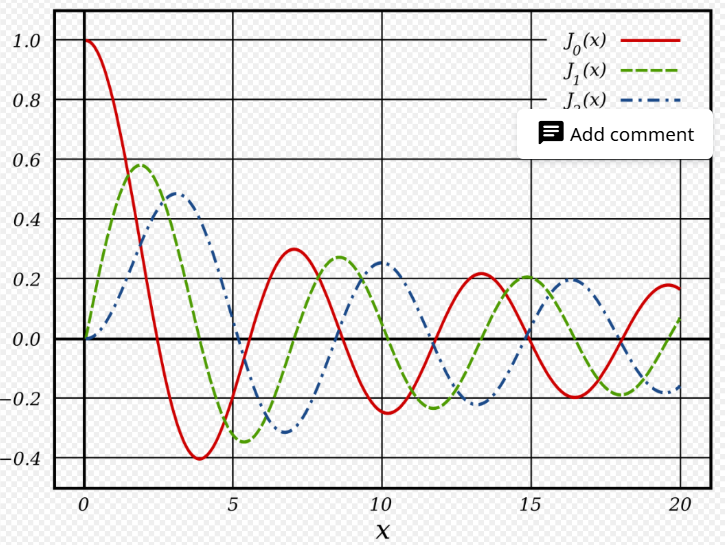
\includegraphics[width=0.5\linewidth]{bessel_functions.png}
    \caption{The first three Bessel functions of the first kind, $J_0$, $J_1$, and $J_2$.}
    \label{fig:bessel_functions}
\end{figure}

For that reason, we want the r-spatial part to be at its peak at r=0, and not 0, which is only satisfied by $J_0(\kappa r)$.

\subsection{Radiative Wall Losses}

At the cylindrical wall $r=R$, radiative energy is lost according to a Marshak-type
Robin boundary condition:
\begin{equation}
\left.
\frac{\partial U}{\partial r}
\right|_{r=R}
=
\frac{3}{4}\rho\kappa_{opacity}(a-1)\,
U(R),
\label{eq::robin_bc}
\end{equation}
where $a$ is the wall albedo.

Using the Bessel function identity (Eq.~\ref{eq::bessel_diff} and Eq.~\ref{eq::bessel_prop})
\[
\frac{d}{dr}J_0(\kappa r) = -\kappa J_1(\kappa r),
\]
the boundary condition yields the eigenvalue equation
\begin{equation}
\boxed{
\kappa_n R J_1(\kappa_n R) = \varepsilon J_0(\kappa_n R),
}
\label{eq::eigenvalue}
\end{equation}
definition of small parameter:
\[
    \varepsilon \equiv \frac{3}{4}(1-a)\tau
\]
where $\tau = \rho\kappa_{opacity} R$ is the optical depth.

Solutions are intersections of: $\kappa R J_1(\kappa R) = \varepsilon J_0(\kappa R)$. 
with small corrections.

This equation determines the discrete spectrum $\{\kappa_n\}$.

\paragraph{Small-loss limit.}
For $\varepsilon \ll 1$, we can express the the zeroth and first bessel functions using their series representation:
\[
J_0(\kappa x) \approx 1 - \frac{ (\kappa x)^2}{4}, \
J_1(\kappa x) \approx \frac{(\kappa x)}{2} - \frac{(\kappa x)^3}{16}.
\]
Substituting into Eq.~\eqref{eq::eigenvalue} we get:
\[
\kappa R \left(\frac{\kappa R}{2} - \frac{(\kappa R)^3}{16}\right) = \varepsilon \left(1 - \frac{ (\kappa R)^2}{4}\right).
\]
or leading order in $\kappa R$,
\[
\frac{(\kappa R)^2}{2} \approx \varepsilon,
\implies \kappa_0 R \approx \sqrt{2\varepsilon}.
\]

---

\section{Marshak Front Representation}

The Marshak front position is expanded in the same radial eigenfunctions:
\begin{equation}
z_F(r,t) =
\sum_{n\ge 0}
c_n(t)\,J_0(\kappa_n r),
\label{eq::front_expansion}
\end{equation}
where $\{\kappa_n\}$ are determined by the Robin wall condition
$\kappa R J_1(\kappa R)=\varepsilon J_0(\kappa R)$.

At leading order, only the lowest mode is retained:
\begin{equation}
z_F(r,t) \approx c_0(t)\,J_0(\kappa_0 r).
\label{eq::leading_front}
\end{equation}

\subsection*{Front Evolution Equation: explicit leading-mode reduction}

We now derive the ODE for $c_0(t)$ from the front energy balance. Following the
Hurricane--Hammer steep-front closure, the front speed is proportional to the
longitudinal radiative flux at the front:
\begin{equation}
\rho e\,\dot{z}_F
=
-\frac{4\sigma}{3\kappa_R \rho}
\left.
\frac{\partial U}{\partial z}
\right|_{z=z_F}.
\label{eq::front_speed}
\end{equation}
Here $\kappa_R$ is the (Rosseland) opacity and $\sigma$ is the Stefan--Boltzmann constant;
$e$ is an effective energy-per-volume parameter for heating the material.

\paragraph{Step 1: leading eigenmode form of $U(z,r,t)$.}
From the separated solution (Eq.~\eqref{eq::general_solution}) we retain only the lowest
radial eigenfunction:
\begin{equation}
U(z,r,t)\approx J_0(\kappa_0 r)\,\Big(A(t)e^{\kappa_0 z}+B(t)e^{-\kappa_0 z}\Big).
\label{eq::U_leading_exp}
\end{equation}

We impose two longitudinal conditions (as in the planar derivation):

\subsection{Source boundary at $z=0$}

From \eqref{eq::general_solution} at $z=0$:
\begin{equation}
T_s^4
=
\sum_{n=0}^{\infty} \big(A_n+B_n\big)\,J_0(k_n r).
\label{eq:source_expand}
\end{equation}
Using orthogonality of $J_0(k_n r)$ on $[0,R]$ with weight $r$, this implies that to leading order only the fundamental mode carries the constant function:
\begin{equation}
A_0+B_0 = T_s^4 + O(\epsilon),\qquad
A_{n\ge 1}+B_{n\ge 1}=O(\epsilon).
\label{eq::AnBn_source}
\end{equation}
(Exactly as in the planar derivation: the constant-in-$r$ boundary drives primarily the lowest mode.)

\subsection{Front boundary condition: weak-curvature implementation (full derivation)}

The bent Marshak front is the moving surface
\[
z=z_F(r,t),
\]
at which the temperature drops sharply. In the steep-front approximation we impose
\[
U\big(z_F(r,t),r,t\big)\approx 0.
\]
Because the wall losses are assumed weak (high albedo), the curvature of the front is small.
We therefore expand the front position about a mean (or centerline) position $c_0(t)$:
\begin{equation}
z_F(r,t)=c_0(t)+\delta z_F(r,t),
\qquad \delta z_F=O(\epsilon).
\label{eq:zF_expand_c0}
\end{equation}

\paragraph{Taylor expansion of the front boundary condition.}
Expand $U(z,r,t)$ about $z=c_0(t)$:
\begin{align}
U\big(z_F(r,t),r,t\big)
&=
U\big(c_0+\delta z_F,r,t\big) \nonumber\\
&=
U(c_0,r,t)
+
\delta z_F(r,t)\,\partial_z U(c_0,r,t)
+\frac{1}{2}\delta z_F(r,t)^2\,\partial_z^2 U(c_0,r,t)
+\cdots.
\label{eq:taylor_front}
\end{align}
Imposing $U(z_F,r,t)\approx 0$ and retaining only the leading term in the weak-curvature limit gives
\begin{equation}
\boxed{
U(c_0,r,t)=0
\qquad\text{(leading order in curvature).}
}
\label{eq::front_leadingBC_full}
\end{equation}
Higher-order corrections can be incorporated by keeping the $\delta z_F\,\partial_z U$ term; here we focus on the leading-order closure.

\paragraph{modal form of the solution in the diffusion region.}
In the quasi-steady diffusion region behind the front, $U$ satisfies Laplace's equation and admits the separated expansion
\begin{equation}
U(z,r,t)=\sum_{n=0}^{\infty} J_0(k_n r)\Big(A_n(t)e^{k_n z}+B_n(t)e^{-k_n z}\Big).
\label{eq::U_series_full}
\end{equation}

\paragraph{impose the leading-order front condition mode-by-mode.}
Insert $z=c_0$ into \eqref{eq::U_series_full} and enforce \eqref{eq::front_leadingBC_full}:
\[
0=U(c_0,r,t)=\sum_{n=0}^{\infty} J_0(k_n r)\Big(A_n e^{k_n c_0}+B_n e^{-k_n c_0}\Big).
\]
Since the set $\{J_0(k_n r)\}$ forms an orthogonal basis on $0\le r\le R$ (with weight $r$), the coefficient of each mode must vanish:
\begin{equation}
\boxed{
A_n(t)e^{k_n c_0(t)}+B_n(t)e^{-k_n c_0(t)}=0
\qquad \forall n.
}
\label{eq:front_mode_condition}
\end{equation}
This immediately gives
\begin{equation}
B_n(t)=-A_n(t)e^{2k_n c_0(t)}.
\label{eq:Bn_in_terms_An}
\end{equation}

\paragraph{rewrite the longitudinal dependence in hyperbolic-sine form.}
Start with the generic $z$-dependence of mode $n$:
\[
A_n e^{k_n z}+B_n e^{-k_n z}.
\]
Substitute \eqref{eq:Bn_in_terms_An}:
\begin{align}
A_n e^{k_n z}+B_n e^{-k_n z}
&=A_n e^{k_n z}-A_n e^{2k_n c_0}e^{-k_n z}\nonumber\\
&=A_n\left(e^{k_n z}-e^{k_n(2c_0-z)}\right)\nonumber\\
&=A_n e^{k_n c_0}\left(e^{k_n(z-c_0)}-e^{-k_n(z-c_0)}\right)\nonumber\\
&=2A_n e^{k_n c_0}\sinh\!\big(k_n(z-c_0)\big).
\label{eq:AB_to_sinh_step}
\end{align}
It is convenient to factor out a normalization $\sinh(k_n c_0)$ so that the remaining coefficient is dimensionless and (later) directly tied to the source boundary condition. Define a new amplitude $\widetilde A_n(t)$ by
\begin{equation}
\widetilde A_n(t)\equiv 2A_n(t)e^{k_n c_0(t)}\,\sinh\!\big(k_n c_0(t)\big).
\label{eq:Atilde_def}
\end{equation}
Then \eqref{eq:AB_to_sinh_step} becomes the compact ``sinh-form''
\begin{equation}
\boxed{
A_n e^{k_n z}+B_n e^{-k_n z}
=
\widetilde A_n(t)\,
\frac{\sinh\!\big(k_n(z-c_0(t))\big)}{\sinh\!\big(k_n c_0(t)\big)}.
}
\label{eq:AB_sinh_form_full}
\end{equation}
This expression automatically satisfies the front condition because at $z=c_0$ the numerator vanishes.

\paragraph{insert back into the full field expansion.}
Substituting \eqref{eq:AB_sinh_form_full} into \eqref{eq::U_series_full} yields
\begin{equation}
U(z,r,t)=
\sum_{n=0}^{\infty}
J_0(k_n r)\,
\widetilde A_n(t)\,
\frac{\sinh\!\big(k_n(z-c_0(t))\big)}{\sinh\!\big(k_n c_0(t)\big)}.
\label{eq::U_sinh_series}
\end{equation}

\paragraph{normalize by the source temperature and define dimensionless amplitudes.}
Let $T_s$ be the imposed source temperature (for constant drive) so that the natural scale is $T_s^4$.
Define dimensionless coefficients
\begin{equation}
\alpha_n(t)\equiv -\frac{\widetilde A_n(t)}{T_s^4}.
\label{eq::alpha_def}
\end{equation}
Then \eqref{eq::U_sinh_series} becomes
\begin{equation}
\boxed{
\frac{U(z,r,t)}{T_s^4}
=
-\sum_{n=0}^{\infty}\alpha_n(t)\,J_0(k_n r)\,
\frac{\sinh\!\big(k_n(z-c_0(t))\big)}{\sinh\!\big(k_n c_0(t)\big)}.
}
\label{eq::U_final_form_full}
\end{equation}
This is exactly the cylindrical analogue of the paper's planar expression (their Eq.~(27)), with $\cos(\cdot)$ replaced by $J_0(\cdot)$ and transverse eigenvalues set by the Robin condition.

\paragraph{how $\alpha_n$ are fixed by the source boundary condition.}
At $z=0$ the boundary condition is $U(0,r,t)=T_s^4$ (constant in $r$ for a uniform drive). Plugging $z=0$ into \eqref{eq::U_final_form_full} gives
\[
1
=
\frac{U(0,r,t)}{T_s^4}
=
-\sum_{n=0}^{\infty}\alpha_n\,J_0(k_n r)\,
\frac{\sinh\!\big(-k_n c_0\big)}{\sinh\!\big(k_n c_0\big)}
=
\sum_{n=0}^{\infty}\alpha_n\,J_0(k_n r),
\]
since $\sinh(-x)=-\sinh(x)$. Therefore
\begin{equation}
\boxed{
1=\sum_{n=0}^{\infty}\alpha_n\,J_0(k_n r)
\qquad (0\le r\le R),
}
\label{eq::alpha_source_match}
\end{equation}
i.e.\ the constant function $1$ is expanded in the $J_0(k_n r)$ basis. This uniquely determines the $\alpha_n$ via Bessel orthogonality (with weight $r$).
In the high-albedo limit, the lowest mode is nearly uniform, so
\[
\alpha_0=1,\qquad \alpha_{n\ge 1}=O(\epsilon),
\]
matching the weak-loss ordering used in the perturbation theory.
Therefore, to leading order we can set $\alpha_0=1$ and $\alpha_{n\ge 1}=0$, giving the leading-mode approximation
\begin{equation}
\boxed{
\frac{U(z,r,t)}{T_s^4} \approx -\alpha_0 J_0(k_0 r) \frac{\sinh(k_0(z-c_0(t)))}{\sinh(k_0 c_0(t))} = J_0(k_0 r) \frac{\sinh(k_0(c_0(t)-z))}{\sinh(k_0 c_0(t))}.
\label{eq::U_hyperbolic}
}
\end{equation}

\paragraph{Step 2: compute the front gradient $\partial_z U|_{z=z_F}$.}
Differentiate \eqref{eq::U_hyperbolic} with respect to $z$:
\begin{align*}
\partial_z U(z,r,t)\approx
U_s(t)\,J_0(\kappa_0 r)\;
\frac{\partial}{\partial z}
\left[
\frac{\sinh(\kappa_0(c_0-z))}{\sinh(\kappa_0 c_0)}
\right]
=\\
-U_s(t)\,J_0(\kappa_0 r)\;
\frac{\kappa_0\cosh(\kappa_0(c_0-z))}{\sinh(\kappa_0 c_0)}.
\end{align*}
Evaluating at the front $z=c_0(t)$ gives
\begin{equation}
\left.\partial_z U\right|_{z=c_0(t)}
\approx
-U_s(t)\,J_0(\kappa_0 r)\;
\frac{\kappa_0}{\sinh\!\big(\kappa_0 c_0(t)\big)}.
\label{eq::dUdz_front}
\end{equation}

\paragraph{Step 3: project the front balance onto the lowest eigenmode.}
Equation \eqref{eq::front_speed} is a \emph{pointwise} statement along the front.
In the leading-mode truncation we enforce it in a weighted (Galerkin) sense by
multiplying both sides by $J_0(\kappa_0 r)$ and integrating over the cross section
with cylindrical weight $r\,dr$:
\begin{equation}
\int_0^R \rho e\,\dot z_F(r,t)\,J_0(\kappa_0 r)\,r\,dr
=
-\frac{4\sigma}{3\kappa_R \rho}
\int_0^R
\left.\partial_z U\right|_{z=z_F}\,
J_0(\kappa_0 r)\,r\,dr.
\label{eq::galerkin}
\end{equation}

Using $z_F(r,t)\approx c_0(t)J_0(\kappa_0 r)$, the left-hand side becomes
\[
\int_0^R \rho e\,\dot c_0(t)\,J_0^2(\kappa_0 r)\,r\,dr
=
\rho e\,\dot c_0(t)\,\mathcal N_0,
\qquad
\mathcal N_0 \equiv \int_0^R J_0^2(\kappa_0 r)\,r\,dr.
\]

Using \eqref{eq::dUdz_front}, the right-hand side becomes
\[
-\frac{4\sigma}{3\kappa_R \rho}
\int_0^R
\left(
-U_s(t)\,J_0(\kappa_0 r)\frac{\kappa_0}{\sinh(\kappa_0 c_0)}
\right)J_0(\kappa_0 r)\,r\,dr
=
\frac{4\sigma}{3\kappa_R \rho}
\frac{U_s(t)\kappa_0}{\sinh(\kappa_0 c_0)}\;\mathcal N_0.
\]

Canceling the common factor $\mathcal N_0$ yields the closed ODE
\begin{equation}
e\,\dot c_0(t)=
\frac{4\sigma}{3\kappa_R \rho^2}\;
\frac{U_s(t)\kappa_0}{\sinh\!\big(\kappa_0 c_0(t)\big)}.
\label{eq::c0_ode_raw}
\end{equation}

\paragraph{Step 4: define an effective diffusion constant $D_M$.}
For a constant drive $U_s(t)=U_0$ (or for slow variation treated quasi-statically),
we define the effective constant
\begin{equation}
D_M \equiv
\frac{8\sigma U_0}{3e\,\kappa_R \rho^2},
\label{eq::D_def}
\end{equation}
so that \eqref{eq::c0_ode_raw} becomes
\begin{equation}
\dot c_0(t)=
\frac{D_M \kappa_0}{2}\,
\frac{1}{\sinh\!\big(\kappa_0 c_0(t)\big)}.
\label{eq::c0_ode}
\end{equation}

\subsection*{Solution for the Isotropic Mode: integration to $\cosh^{-1}$}

Multiply \eqref{eq::c0_ode} by $\kappa_0\sinh(\kappa_0 c_0)$:
\[
\kappa_0\sinh(\kappa_0 c_0)\,\dot c_0
=
\frac{D_M \kappa_0^2}{2}.
\]
Recognizing the left-hand side as a time derivative,
\[
\frac{d}{dt}\cosh(\kappa_0 c_0)
=
\kappa_0\sinh(\kappa_0 c_0)\,\dot c_0,
\]
we obtain
\begin{equation}
\frac{d}{dt}\cosh(\kappa_0 c_0)=\frac{D_M \kappa_0^2}{2}.
\end{equation}
Integrating from $t=0$ with $c_0(0)=0$ gives
\[
\cosh(\kappa_0 c_0(t)) = 1 + \frac{D_M \kappa_0^2 t}{2}.
\]
Therefore,
\begin{equation}
\boxed{
c_0(t)
=
\frac{1}{\kappa_0}
\cosh^{-1}
\left(
1 + \frac{D_M \kappa_0^2\,t}{2}
\right).
}
\label{eq::c0_solution}
\end{equation}

Finally, the leading-order front shape is
\begin{equation}
\boxed{
z_F(r,t)
\approx c_0(t)\,J_0(\kappa_0 r)
=
\frac{1}{\kappa_0}
\cosh^{-1}
\left(
1 + \frac{D_M \kappa_0^2\,t}{2}
\right)
J_0(\kappa_0 r).
}
\end{equation}

One can make the derivation even better if defining $D = D_M (1+\frac{\varepsilon}{2})$ (higher order accuracy):
\begin{equation}
\boxed{
z_F(r,t)
\approx c_0(t)\,J_0(\kappa_0 r)
=
\frac{1}{\kappa_0}
\cosh^{-1}
\left(
1 + \frac{D \kappa_0^2\,t}{2}
\right)
J_0(\kappa_0 r).
}
\end{equation}

\subsection*{Time-dependent drive $U_s(t)$ (non-constant boundary temperature)}

So far, the closed-form solution \eqref{eq::c0_solution} was obtained assuming a
\emph{constant} drive $U_s(t)=U_0$ (equivalently, constant boundary temperature
$T_s$ so that $U_s=T_s^4$). We now generalize the derivation to an \emph{arbitrary}
time-dependent drive $U_s(t)$.

\paragraph{Where $U_s(t)$ enters.}
The only place where the drive appears in the leading-mode reduction is through the
boundary condition at $z=0$,
\[
U(0,r,t)=U_s(t),
\]
which implies $A(t)+B(t)=U_s(t)$ (Eq.~\eqref{eq::AnBn_source}). Repeating the same algebra as
in \eqref{eq::dUdz_front} (with $U_0\to U_s(t)$), we obtain the
front gradient
\begin{equation}
\left.\partial_z U\right|_{z=c_0(t)}
\approx
-U_s(t)\,J_0(\kappa_0 r)\;
\frac{\kappa_0}{\sinh\!\big(\kappa_0 c_0(t)\big)}.
\label{eq::dUdz_front_time_drive}
\end{equation}
Therefore, the Galerkin projection step (Eq.~\eqref{eq::galerkin}) yields the same ODE
structure as before, but with an explicit $U_s(t)$ factor:
\begin{equation}
\dot c_0(t)=
\frac{\kappa_0}{\sinh\!\big(\kappa_0 c_0(t)\big)}\;
\frac{4\sigma}{3e\,\kappa_R\rho^2}\;U_s(t).
\label{eq::c0_ode_time_drive_raw}
\end{equation}

\paragraph{Define a time-dependent diffusion coefficient.}
It is convenient to define
\begin{equation}
D_M(t)\equiv \frac{8\sigma}{3e\,\kappa_R\rho^2}\,U_s(t),
\label{eq::DM_time_def}
\end{equation}
so that Eq.~\eqref{eq::c0_ode_time_drive_raw} becomes
\begin{equation}
\dot c_0(t)=
\frac{D_M(t)\,\kappa_0}{2}\,
\frac{1}{\sinh\!\big(\kappa_0 c_0(t)\big)}.
\label{eq::c0_ode_time_drive}
\end{equation}

\paragraph{Integration for general $U_s(t)$.}
Multiply Eq.~\eqref{eq::c0_ode_time_drive} by $\kappa_0\sinh(\kappa_0 c_0)$ to obtain
\[
\frac{d}{dt}\cosh(\kappa_0 c_0(t))=\frac{\kappa_0^2}{2}\,D_M(t).
\]
Integrating from $0$ to $t$ with $c_0(0)=0$ gives
\begin{equation}
\boxed{
\cosh\!\big(\kappa_0 c_0(t)\big)
=
1+\frac{\kappa_0^2}{2}\int_0^t D_M(t')\,dt'
=
1+\frac{4\sigma\,\kappa_0^2}{3e\,\kappa_R\rho^2}\int_0^t U_s(t')\,dt'.
}
\label{eq::cosh_general_drive}
\end{equation}
Hence,
\begin{equation}
\boxed{
c_0(t)=\frac{1}{\kappa_0}\cosh^{-1}\!\left(
1+\frac{\kappa_0^2}{2}\int_0^t D_M(t')\,dt'
\right)
=
\frac{1}{\kappa_0}\cosh^{-1}\!\left(
1+\frac{4\sigma\,\kappa_0^2}{3e\,\kappa_R\rho^2}\int_0^t U_s(t')\,dt'
\right).
}
\label{eq::c0_general_drive}
\end{equation}

Finally, the leading-order cylindrical front shape becomes
\begin{equation}
\boxed{
z_F(r,t)\approx c_0(t)\,J_0(\kappa_0 r)
=
\frac{J_0(\kappa_0 r)}{\kappa_0}\cosh^{-1}\!\left(
1+\frac{4\sigma\,\kappa_0^2}{3e\,\kappa_R\rho^2}\int_0^t U_s(t')\,dt'
\right).
}
\label{eq::zF_general_drive}
\end{equation}

\paragraph{Special case: power-law drive.}
If $U_s(t)=U_0\left(\frac{t}{t_0}\right)^p$ for $t\ge 0$, then
\[
\int_0^t U_s(t')\,dt' = \frac{U_0}{p+1}\frac{t^{p+1}}{t_0^p},
\]
and Eq.~\eqref{eq::c0_general_drive} becomes
\[
c_0(t)=\frac{1}{\kappa_0}\cosh^{-1}\!\left(
1+\frac{4\sigma\,\kappa_0^2}{3e\,\kappa_R\rho^2}\cdot
\frac{U_0}{p+1}\frac{t^{p+1}}{t_0^p}
\right).
\]
This reduces to the constant-drive expression when $p=0$.


---

\section{Physical Interpretation}

\begin{itemize}
\item The transverse structure is governed by $J_0(\kappa_0 r)$ rather than $\cos(k_0 y)$.
\item Radiative wall losses introduce curvature and retard the front.
\item Cylindrical geometry enhances edge cooling relative to planar geometry.
\item The leading-order dynamics are entirely controlled by the lowest eigenvalue $\kappa_0$.
\end{itemize}

The correspondence between planar and cylindrical formulations is:
\[
\cos(k y)
\;\longleftrightarrow\;
J_0(\kappa r),
\qquad
\tan(kL)
\;\longleftrightarrow\;
\frac{\kappa R J_1(\kappa R)}{J_0(\kappa R)}.
\]

All higher-order perturbation theory carries over with this substitution.

\section{Usful bessel function identities}
Series Representation:
\begin{equation}
J_n(x) = \sum_{m=0}^{\infty} \frac{(-1)^m}{m! \, \Gamma(m+n+1)} \left(\frac{x}{2}\right)^{2m+n}
\end{equation}
Proparties: 
\begin{equation}
2nJ_n(x) = x(J_{n-1}(x) + J_{n+1}(x))
\end{equation}
\begin{equation}
J_n(-x) = (-1)^n J_n(x), \quad
J_{-n} = (-1)^n J_n(x)
\label{eq::bessel_prop}
\end{equation}
Differentiation, 
\begin{equation}
\frac{d}{dx} J_n(x) = \frac{1}{2}(J_{n-1}(x) - J_{n+1}(x))
\label{eq::bessel_diff}
\end{equation}
\begin{equation}
\frac{d}{dx} \left[x^n J_n(x)\right] = x^n J_{n-1}(x), \qquad \frac{d}{dx} \left[x^{-n} J_n(x)\right] = -x^{-n} J_{n+1}(x)
\end{equation}
Asymptotic form for large and small x:
\begin{equation}
J_n(x) \approx \frac{1}{n!} \left(\frac{x}{2}\right)^n, \quad x \ll 1
\end{equation}
\begin{equation}
J_n(x) \approx \sqrt{\frac{2}{\pi x}} \cos\left(x - \frac{n\pi}{2} - \frac{\pi}{4}\right), \quad x \gg 1
\end{equation}
And lastly the orthogonality relation:
\begin{equation}
\int_0^R r J_n\left(\frac{\alpha_{m} r}{R}\right) J_n\left(\frac{\alpha_{k} r}{R}\right) dr = \frac{R^2}{2} \left[J_{n+1}(\alpha_{m})\right]^2 \delta_{mk}
\end{equation}
where $\alpha_m$ is the m'th root of $J_n(x)$.

\section*{Albedo Derivation}

Consider a gold cylindrical shell surrounding foam.

Let

\begin{align}
F_{\text{in}} &= \sigma_{SB} T_s^4 \\
F_{\text{out}} &= \sigma_{SB} T_{\text{obs}}^4
\end{align}

The detector measures the re-emitted flux:

\begin{equation}
\sigma_{SB} T_{\text{obs}}^4
=
\sigma_{SB} T_s^4
+
\frac{F(0,t)}{2}
\end{equation}

Thus,

\begin{equation}
\sigma_{SB} T_s^4
-
\frac{F(0,t)}{2}
=
\sigma_{SB} T_{\text{obs}}^4
\end{equation}

Since

\begin{equation}
F(0,t) = \dot{E}_w
\end{equation}

we define the albedo:

\begin{equation}
a(t)
=
\frac{\text{reflected flux}}{\text{incident flux}}
=
\frac{F_{\text{in}}}{F_{\text{out}}}
=
\frac{
\sigma_{SB} T_0^4 + \frac{\dot{E}_w}{2}
}{
\sigma_{SB} T_0^4 - \frac{\dot{E}_w}{2}
}
\end{equation}

\end{document}